\documentclass[a4paper]{article}

\usepackage[english]{babel}
\usepackage[utf8]{inputenc}
\usepackage{amsmath}
\usepackage{graphicx}
\usepackage[colorinlistoftodos]{todonotes}
\usepackage{bm,amsmath,subfigure}

\title{CS 543 - Assignment 1: Shape from Shading }

\author{Yiwen Xu}

\date{\today}

\begin{document}
\maketitle

\begin{abstract}
This project mainly accomplished the task to reconstruct faces from a series of pictures of taken under different illuminants. Based on \textbf{Photometric stereo},
surface normals are reconstructed after basic per-processing of image series and integration is applied on surface normals to form the height map.
\end{abstract}

% --------------------------------------------------------
\section{Description of Implementation}
\label{sec:introduction}

\subsection{Albedo and Surface Normals Estimation}
When solving least square problems for albedo and surface normal, instead of directly implement the method introduced in the lecture, some adjustments have been made to improve the performance. In order to avoid loops in Matlab, the least square problem is arranged in following way so that all can be solved at one backslash operation.
\begin{flushleft}
$
\begin{bmatrix}
    I_{1}(x_{1},y_{1}) & I_{1}(x_{2},y_{2}) & \cdots  & I_{1}(x_{lm},y_{lm}) \\
    I_{2}(x_{1},y_{1}) & I_{2}(x_{2},y_{2}) & \cdots  & I_{2}(x_{lm},y_{lm}) \\
    \vdots 			   & \vdots  			& \ddots  & \vdots			     \\
    I_{n}(x_{1},y_{1}) & I_{n}(x_{2},y_{2}) & \cdots  & I_{n}(x_{lm},y_{lm}) \\
\end{bmatrix}_{n \times (l \times m)}
$
\end{flushleft}

\begin{flushright}
$
=\begin{bmatrix}
    V_{1} \\
    V_{2} \\
    \vdots\\ 
    V_{n} \\ 
\end{bmatrix}_{n \times 3}
\begin{bmatrix}
	g(x_{1},y_{1}) & g(x_{2},y_{2}) & \cdots & g(x_{lm},y_{lm}) \\ 
\end{bmatrix}_{3 \times lm}
$
\end{flushright}

\subsection{Height Map Recover}
Five implementation of integration methods to recover height map is implemented, namely 'Column', 'Row', 'Average', 'Random' and 'Onedim-Random'.

{\bfseries{\em Column, Row and Average:}} Take 'Column' as an example, integration is accomplished by first generate integration along the first column and than take the integrated first row as a start to accumulate row-wisely. 'Row' is implemented likewise and 'Average' is simply the mean of 'Row' and 'Column'.

{\bfseries{\em Random Path:}} Random path implementation start from the leftup corner and randomly select path to go vertically and horizontally towards destination $(x,y)$. Direction could be changed at each pixel.

{\bfseries{\em One Dimensional Random Path:}} Randomly pick one row as start and divide the image into two parts, namely upper one and lower one, then integrate vertically in different direction. This method is plus method to eliminate distortions due to long accumulation path.

\subsection{Artifacts and Limitations}
One artifacts with my implementation of random path would be the non-smooth surface in the rightdown corner.The reason for this might be the directions turn too frequently. For a small area, if neighboring pixels accumulated from dramatically different paths which carry dramatically different errors. these error cannot be eliminated by simply averaging. Details explained in latter section.

% --------------------------------------------------------
\section{Integration Methods}
\label{sec:integration}

\subsection{Output Comparison}
Given to the experience I have conducted, I would say 'Column' works best among four basic types of integration methods. Output height map from different methods are shown in Figure \ref{fig:comp_int}.

{\bfseries{\em Reason of Difference:}} 

In my understanding, the quality of height map largely depend on the travel distance that carrying errors. The longer distance as it travels the poorer quality that area is going to get. The most significant error in the face comes from parts under nose when going vertically down. Therefore, 'Row' start with initial row at top and takes large accumulated error as it travel downwards especially under nose part. In contrast to 'Column', where the vertical big error is avoided by traveling horizontal rightwards across that part and thus make quality height map. The 'Average' takes the wavy lip from 'Row' and mix with 'Column' thus has quality in between. 

Another issue affects quality of height map comes from the travel path coherency in neighboring area. When using 'Random', neighboring pixels is going to be integrated from significant different path. As it is seen in comparison, errors at same area can be different when travel in different directions. Therefore frequent turning direction makes huge difference between neighboring pixels. Averaging somehow  doesn't make up for the accumulated error. Assume we are traveling from $(m,n)$ to $(m,n+k)$, even if the latter point coming from subpath of former one, there is going to be $2^{k}$ methods of afterwards steps. As the averaging effects grows linearly, the error grows exponentially. Therefore in random right-down corner has more profound artifacts.

\begin{figure}[h!]
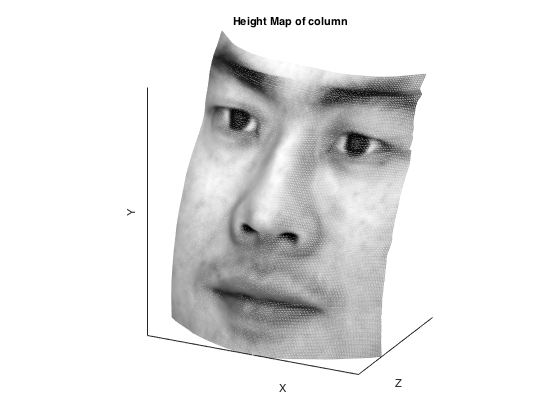
\includegraphics[width=0.6\textwidth]{imgs/2col.png}
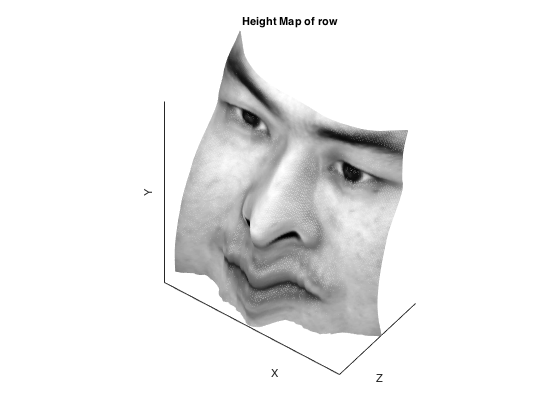
\includegraphics[width=0.6\textwidth]{imgs/2row.png}
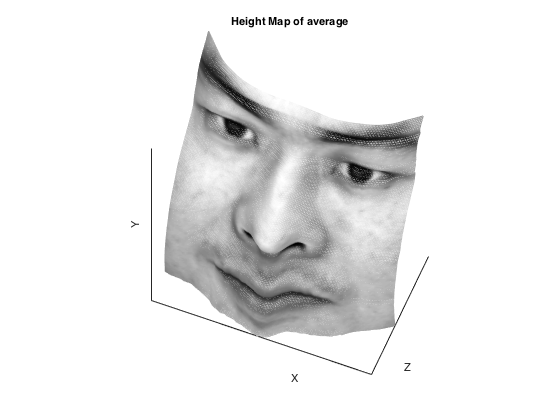
\includegraphics[width=0.6\textwidth]{imgs/2ave.png}
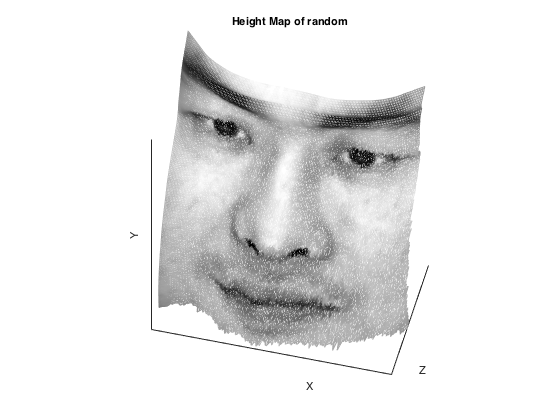
\includegraphics[width=0.6\textwidth]{imgs/2ran.png}
\caption{\label{fig:comp_int} Output height maps from 4 basic methods, namely 'Column', 'Row', 'Average' and 'Random'.}
\end{figure}


\subsection{Running Time}
The running time of four basic methods as well as my additional implementation of 'One-dimensional Random' is shown in Table \ref{tab:runtime}.

\begin{table}[h!]
\centering
\begin{tabular}{l|rrrrr}
Implementation & Column & Row & Average & Random & One-dim Random \\\hline
Running Time & 5.8349e-04 & 6.7812e-04 & 0.0011 & 0.7571 & 0.0058 \\
\end{tabular}
\caption{\label{tab:runtime}The running time comparison for different implementation.}
\end{table}

\subsection{Additional Illustration}
For other subjects, generally speaking column is still the best but sometimes chins could wrongly go upwards. The best output of rest of subject shown as Figure \ref{fig:addi}.

\begin{figure}[h!]
\minipage{0.32\textwidth}
  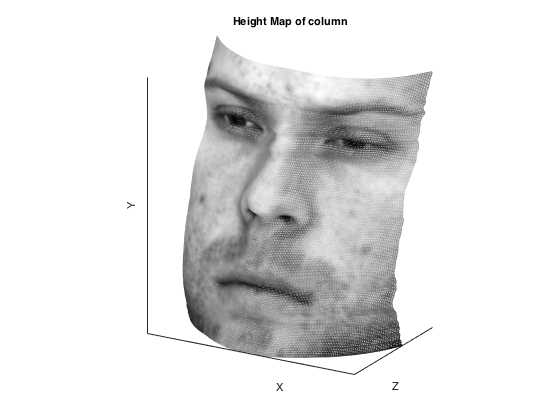
\includegraphics[width=\linewidth]{imgs/1col.png}
\endminipage\hfill
\minipage{0.32\textwidth}
  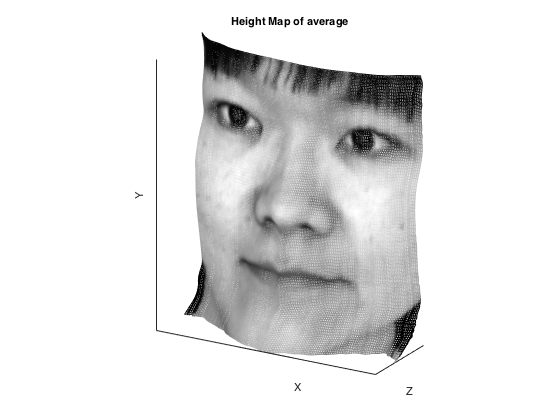
\includegraphics[width=\linewidth]{imgs/5aver.png}
\endminipage\hfill
\minipage{0.32\textwidth}%
  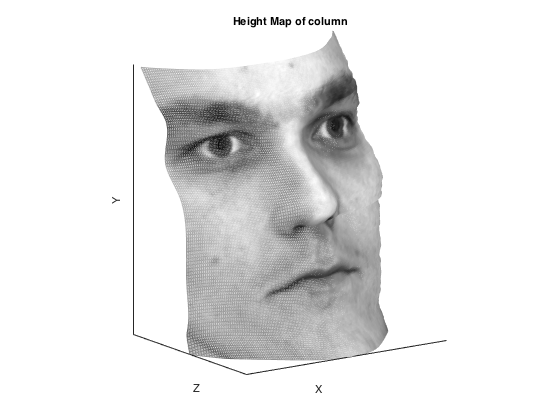
\includegraphics[width=\linewidth]{imgs/7col.png}
\endminipage
\caption{\label{fig:addi} Best output height maps from rest of subjects.}
\end{figure}

% --------------------------------------------------------
\section{Albedo and Height Maps}
The estimated albedo maps, surface normals and height maps for each subject is shown in Figure \ref{fig:out}. The 3D height maps is constructed all in 'Column' method for comparison. As one can see,
'Column' is not necessarily the best integration method for subject 5 where creates an obvious up-pointed chin. Improvement will be introduce in next section.

\begin{figure}[h!]
\centering
\subfigure[3D]{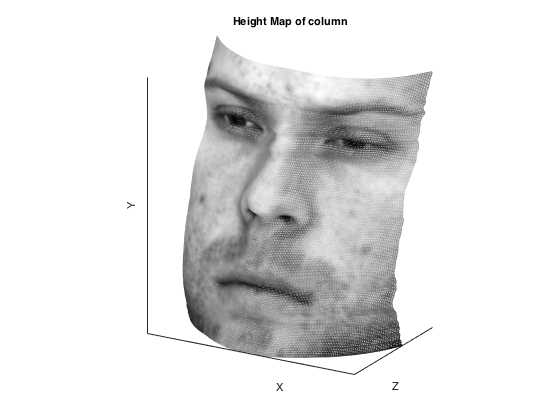
\includegraphics[width= 0.2\textwidth]{imgs/1col.png}}
\subfigure[Albedo]{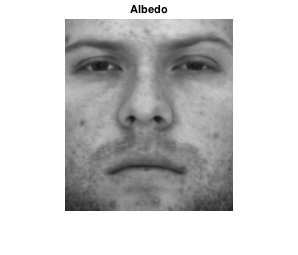
\includegraphics[width= 0.2\linewidth]{imgs/1abd.png}}
\subfigure[Surface Normals]{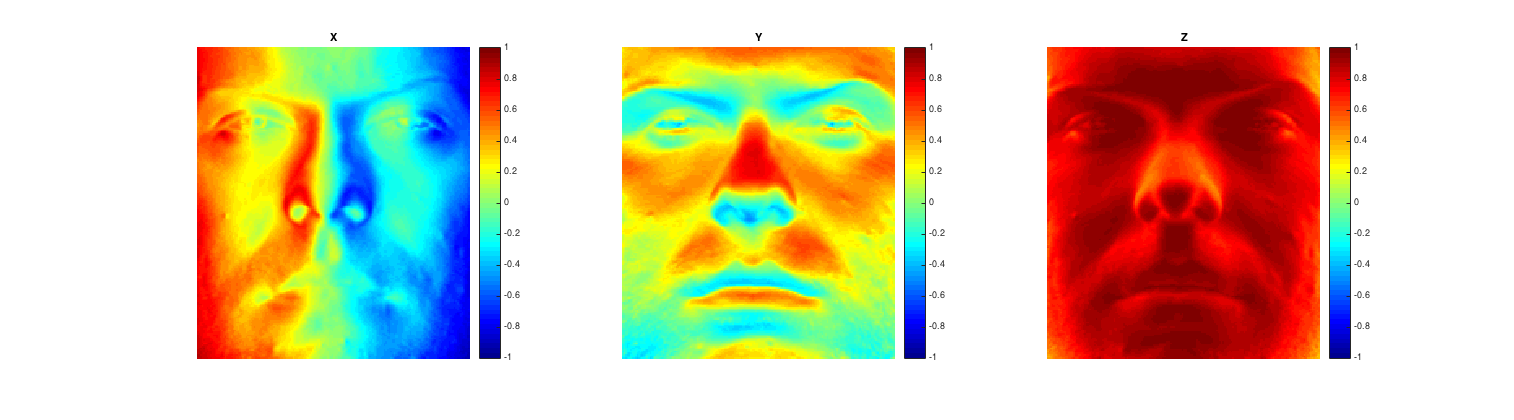
\includegraphics[width= 0.58\linewidth]{imgs/1sn.png}}
\centering
\subfigure[3D]{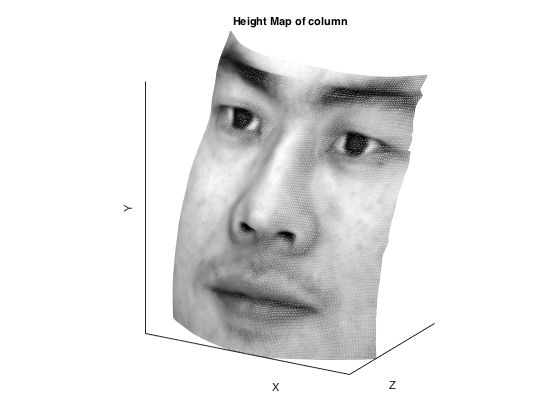
\includegraphics[width= 0.2\textwidth]{imgs/2c.png}}
\subfigure[Albedo]{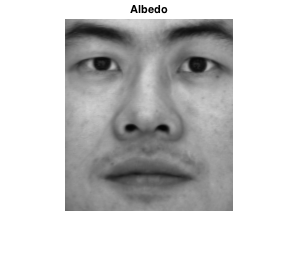
\includegraphics[width= 0.2\linewidth]{imgs/2abd.png}}
\subfigure[Surface Normals]{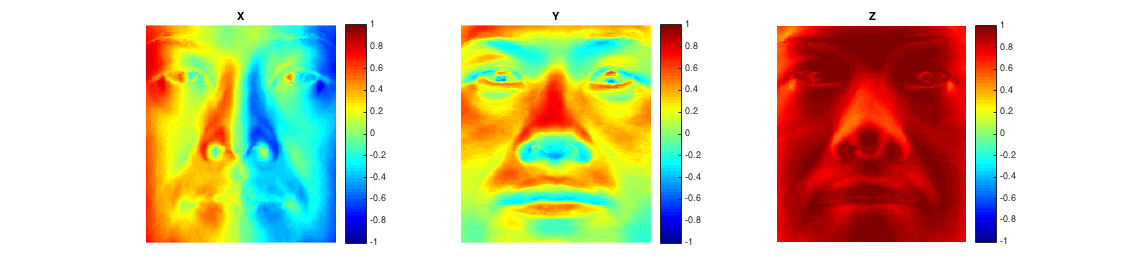
\includegraphics[width= 0.58\linewidth]{imgs/2sn.png}}
\centering
\subfigure[3D]{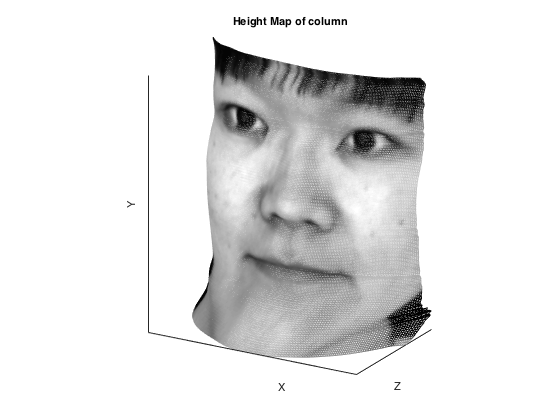
\includegraphics[width= 0.2\textwidth]{imgs/5c.png}}
\subfigure[Albedo]{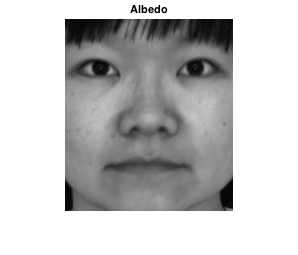
\includegraphics[width= 0.2\linewidth]{imgs/5abd.png}}
\subfigure[Surface Normals]{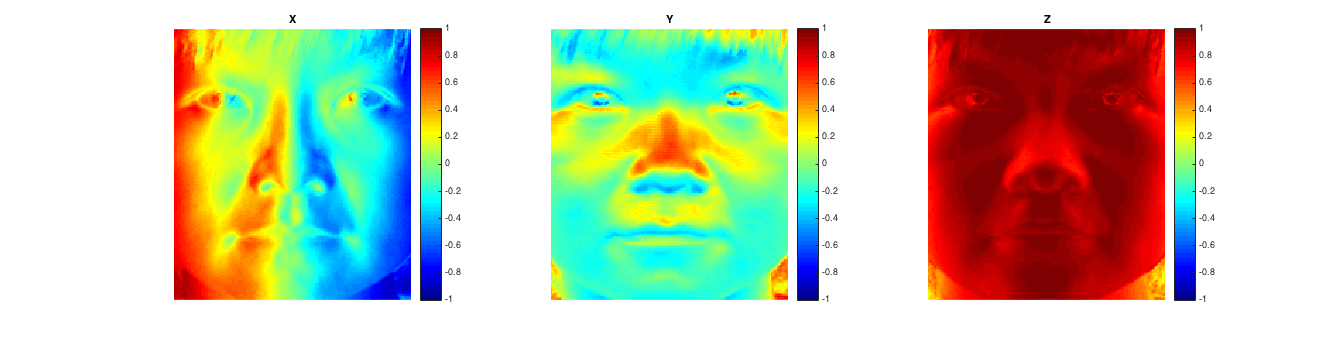
\includegraphics[width= 0.58\linewidth]{imgs/5sn.png}}
\centering
\subfigure[3D]{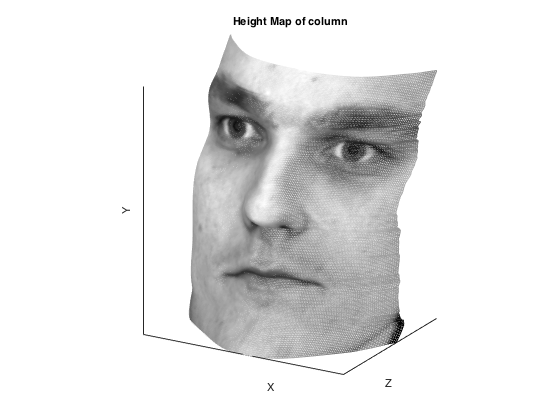
\includegraphics[width= 0.2\textwidth]{imgs/7c.png}}
\subfigure[Albedo]{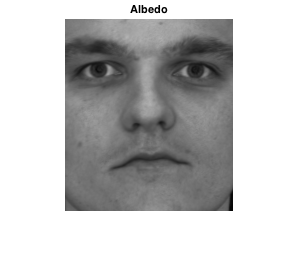
\includegraphics[width= 0.2\linewidth]{imgs/7abd.png}}
\subfigure[Surface Normals]{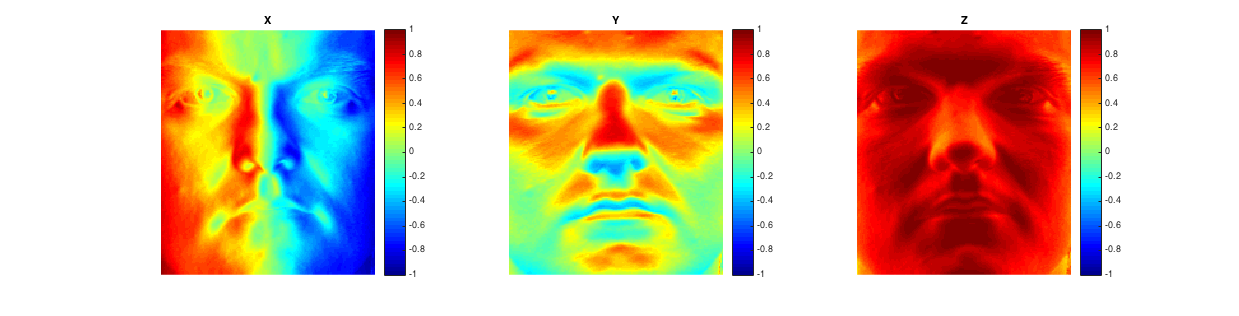
\includegraphics[width= 0.58\linewidth]{imgs/7sn.png}}
\caption{3D, albedo and surface normal maps for subject 1,2,5,7\label{fig:out}}
\end{figure}

% --------------------------------------------------------
\section{Improvement for Extra Credit}
As it is mentioned in former section, the estimated error of height maps is accumulative thus its quality highly depend on traveling distance. Common problems for subject 5 and 7 is that they probably contain up-pointing chins. The reason for that is the long distance accumulation of error area, most errors happens in under nose part. 

\subsection{One dimensional random}
In this section, One dimensional random method is introduced to eliminate the error by decrease accumulating distance. To do that, a random horizontal line is picked as initial constant. In this line each pixel is integrated from left to right. For the vertical direction, integration happens from the initial line and go up or down towards target position. When go upwards, the integration happens reversely travel from down to up with negative value for the middle random line is considered as a hill. When go downwards, the integration happens normally.
\subsection{Output Improvements}
Comparison between 'Column' and 'One dimensional Random' shown in Figure \ref{fig:imp}. As a matter of face, one dimensional random method generally overperforms other basic method in creating overall good estimation but still contains some artifacts like wavy surface.
\begin{figure}[h!]
\centering
\subfigure[Basic Column]{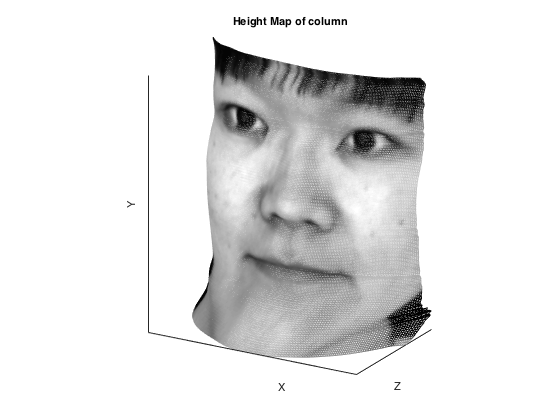
\includegraphics[width= 0.32\textwidth]{imgs/5c.png}}
\subfigure[Onedim Random]{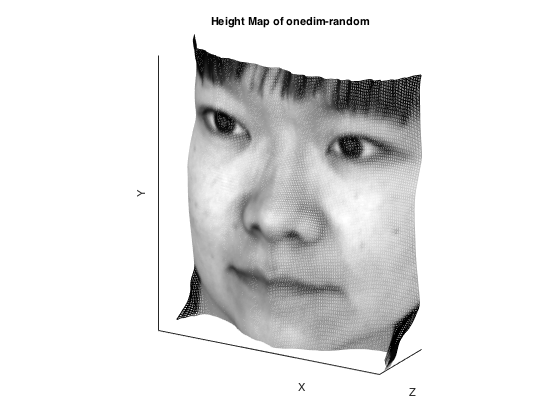
\includegraphics[width= 0.32\linewidth]{imgs/5od.png}}
\subfigure[Onedim (side view)]{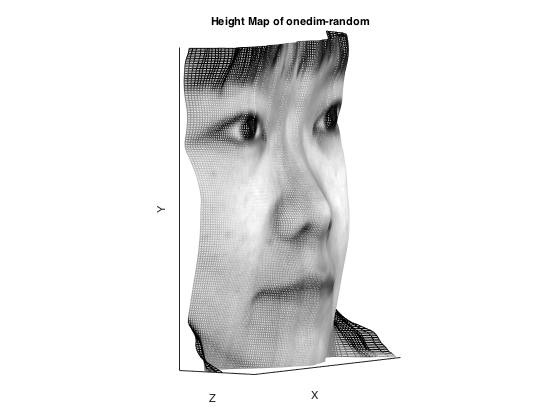
\includegraphics[width= 0.32\linewidth]{imgs/5od2.png}}
\centering
\subfigure[Basic Column]{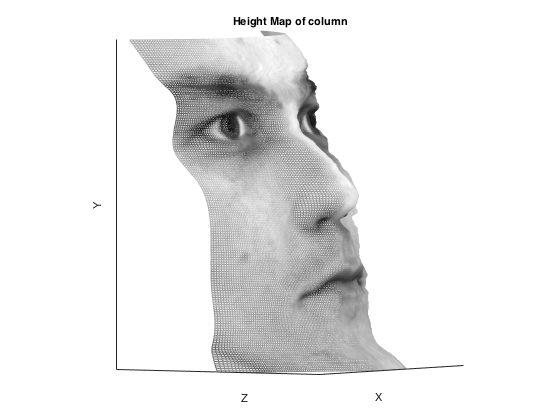
\includegraphics[width= 0.32\textwidth]{imgs/7co.png}}
\subfigure[Onedim Random]{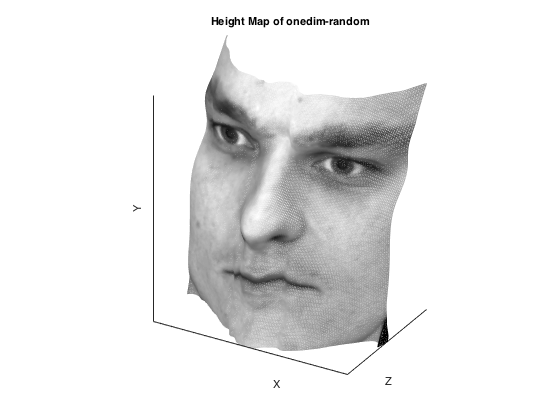
\includegraphics[width= 0.32\linewidth]{imgs/7od1.png}}
\subfigure[Onedim (side view)]{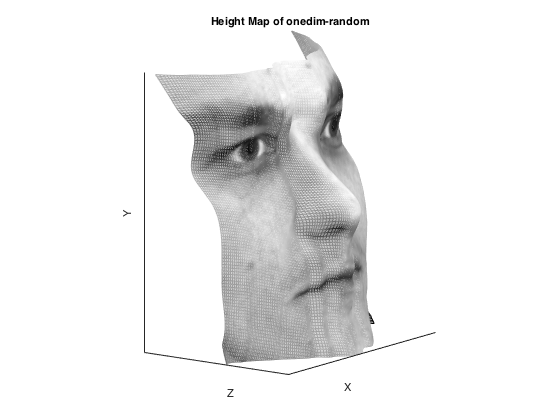
\includegraphics[width= 0.32\linewidth]{imgs/7od.png}}
\caption{Output improvement for subject 5,7 using one dimensional random\label{fig:imp}}
\end{figure}
% --------------------------------------------------------
\section{Discussion}
\subsection{Violate of Assumption}
There are Shape from shading method based on the assumption that pixel value of pictures follows Lambert's law of diffuse reflection. In the diffusive reflection,light should be reflected equally in all directions and independent of viewing direction. 

However,such assumption is not satisfied with the image input.Take subjects 1 as an illustration. Human skin is not a perfect object of diffuse reflection due to oils in the face. Numbers of input image actually contains huge amount of specular reflection which is much brighter than diffuse reflection and dependent on viewing directions, such as images shown in Figure \ref{fig:vio}. Those specular reflection might cause that area much higher than it supposed to be. So generally nose with specular light looks higher.

Also, the change of facial expression also have something to do with the final accuracy since the person is not always stable.In addition, eyebrow parts also create problems because they are furry and somehow eliminate the reflecting lights. In the model, therefore eyebrow more likely to be concave parts.

\begin{figure}[h!]
\centering
\subfigure[Nose]{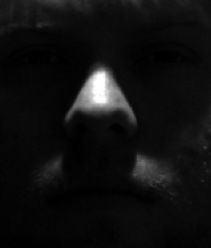
\includegraphics[width= 0.32\textwidth]{imgs/1vio.jpg}}
\subfigure[Front head]{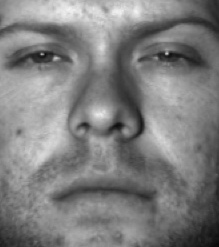
\includegraphics[width= 0.32\linewidth]{imgs/2vio.jpg}}
\subfigure[Change expression]{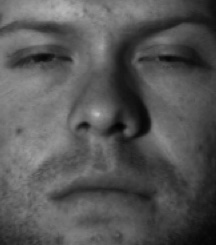
\includegraphics[width= 0.32\linewidth]{imgs/3vio.jpg}}
\caption{Sample images of violation\label{fig:vio}}
\end{figure}

As for using subset to improve quality of face, I tried with several subset of images getting rid of problematic images but no significant improvement is found, though.
% --------------------------------------------------------
\begin{thebibliography}{12}
\bibitem{nano3}
 David A. Forsyth, Jean Ponce 
  \emph{Computer Vision: A Modern Approach, 2nd Edition}.
  
\bibitem{nano3}
Yale Face dataset
  \emph{http://www.cad.zju.edu.cn/home/dengcai/Data/FaceData.html}.

\bibitem{nano3}
Lecture Notes, Svetlana Lazebnik
	\emph{http://slazebni.cs.illinois.edu/spring16/lec04\_light.pdf}.
    
\end{thebibliography}
\end{document}